% !TEX TS-program = pdflatex
% !TEX encoding = UTF-8 Unicode

\documentclass[a4paper, titlepage=false, parskip=full-, 10pt]{scrartcl}

\usepackage[utf8]{inputenc}
\usepackage[T1]{fontenc}
\usepackage[english, ngerman]{babel}
\usepackage{babelbib}
\usepackage{hyperref}
\usepackage{listings}
\usepackage{framed}
\usepackage{color}
\usepackage{graphicx}
\usepackage[normalem]{ulem}
\usepackage{cancel}
\usepackage{amsmath}
\usepackage{amssymb}
\usepackage{amsthm}
\usepackage{algorithm}
\usepackage{algorithmic}
\usepackage{geometry}
\usepackage{subfigure}
\geometry{a4paper, top=20mm, left=35mm, right=25mm, bottom=40mm}

\newcounter{tasknbr}
\setcounter{tasknbr}{1}
\newenvironment{task}[1]{{\bf Aufgabe \arabic {tasknbr}\stepcounter{tasknbr}} (#1):\begin{enumerate}}{\end{enumerate}}
\newcommand{\subtask}[1]{\item[#1)]}

% Listings -----------------------------------------------------------------------------
\definecolor{red}{rgb}{.8,.1,.2}
\definecolor{blue}{rgb}{.2,.3,.7}
\definecolor{lightyellow}{rgb}{1.,1.,.97}
\definecolor{gray}{rgb}{.7,.7,.7}
\definecolor{darkgreen}{rgb}{0,.5,.1}
\definecolor{darkyellow}{rgb}{1.,.7,.3}
\lstloadlanguages{C++,[Objective]C,Java}
\lstset{
escapeinside={§§}{§§},
basicstyle=\ttfamily\footnotesize\mdseries,
columns=fullflexible, % typewriter font look better with fullflex
keywordstyle=\bfseries\color{blue},
% identifierstyle=\bfseries,
commentstyle=\color{darkgreen},      
stringstyle=\color{red},
numbers=left,
numberstyle=\ttfamily\scriptsize\color{gray},
% stepnumber=5,
% numberfirstline=true,
breaklines=true,
% prebreak=\\,
showstringspaces=false,
tabsize=4,
captionpos=b,
% framexrightmargin=-.2\textwidth,
float=htb,
frame=tb,
frameshape={RYR}{y}{y}{RYR},
rulecolor=\color{black},
xleftmargin=15pt,
xrightmargin=4pt,
aboveskip=\bigskipamount,
belowskip=\bigskipamount,
backgroundcolor=\color{lightyellow},
extendedchars=true,
belowcaptionskip=15pt}

%% Enter current values here: %%
\newcommand{\lecture}{Algorithmische Geometrie SS15}
\newcommand{\tutor}{}
\newcommand{\assignmentnbr}{3}
\newcommand{\students}{Julius Auer, Alexa Schlegel}
%%-------------------------------------%%

\begin{document}  
\lstset{language=Java}
{\small \textsl{\lecture \hfill \tutor}}
\hrule
\begin{center}
\textbf{Übungsblatt \assignmentnbr}\\
[\bigskipamount]
{\small \students}
\end{center}
\hrule

\begin{task}{Graham-Scan}\item[]
Implementieren Sie den Graham-Scan. Benutzen Sie dabei aus Gründen besserer Laufzeit und zur Vermeidung von Rundungsfehlern möglichst nur die Grundrechenarten $+,-,\times, \div$. Eine Umrechnung in Polarkoordinaten, wie in der Vorlesung beschrieben, ist nicht nötig, um die Strahlen nach Steigung zu sortieren.

Im Folgenden wird der Algorithmus beschrieben, welcher implementiert wurde. Er orientiert sich an der in \emph{Introduction to Algorithms}\footnote{Introduction to Algorithms, Second Edition, S. 949}. Der Stack $S$ wird verwendet, um mögliche Kandidaten der konvexen Hülle abzulegen. Terminiert der Algorithmus so enthält $S$ die Knoten der konvexten Hülle, gegen den Urzeigersinn.

\begin{algorithm}
\caption{Graham-Scan(Q)}
\begin{algorithmic}[1]
\STATE sei $p_0 \in Q$ mit minimaler $y$-Koordinate:
bei gleicher $y$-Koordinate minimale $x$-Koordinate verwenden
\STATE sei ${p_1, p_2, \dots, p_n}$ die restlichen Punkte aus $Q$:\\
sortiert nach Polarkooridaten\\
gegen den Urzeigersinn\\
bei gleichem Winkel, nur den Punkt behalten der den größten Abstand von $p_0$ hat\\
(TODO schauen wie das ohne Polarkoordinaten auch geht, evtl. Kreuzprodukt oder so)\\
\STATE \textsc{Push}($p_0$, $S$)\\
\STATE \textsc{Push}($p_1$, $S$)\\
\STATE \textsc{Push}($p_2$, $S$)\\
\FOR{$i=3$ \TO $n$}
    \WHILE{Winkel (\textsc{Next-To-Top}($S$), \textsc{Top}($S$), $p_i$) ist keine Linkskurve}
    \STATE \textsc{Pop}($S$)
    \ENDWHILE
    \STATE \textsc{Push}($p_1$, $S$)
\ENDFOR
\RETURN{$S$}
\end{algorithmic}
\end{algorithm}

\begin{lstlisting}
\end{lstlisting}
\end{task}

\begin{task}{inkrementelle Konstruktion der konvexen Hülle}\item[]
Die ersten drei Punkte $S=p_1,p_2,p_3$ werden zunächst nach X-Koordinate aufsteigend und dann nach Y-Koordinate absteigend sortiert. Die konvexe Hülle $CH(S)=S$ ist somit ein Polygonzug der im Uhrzeigersinn verläuft. Ferner wird das Center of Mass $com=((x_1+x_2+x_3)/3,(y_1+y_2+y_3)/3)$ bestimmt. Außerdem wird als Datenstruktur ein binärer Suchbaum $T$ angelegt, der $search(p)$, $insert(p)$ und $delete(p)$ in $O(\log n)$ garantiert (z.B. ein AVL-Baum) - in diesen werden $p_1,p_2,p_3$ eingefügt, wobei die totale Ordnung gegeben ist durch
$$p_i<p_j\text{ g.d.w. }\frac{y_i-y_{com}}{x_i-x_{com}}<\frac{y_j-y_{com}}{x_j-x_{com}}$$
wenn also die Steigung zwischen $com$ und $p_i$ kleiner ist, als die von $com$ und $p_j$. Diese Ordnung gilt auch für zukünftige Operationen auf dem Baum. $search(p)$ soll hierbei den Punkt aus $CH(S)$ liefern, der die nächst kleinere Steigung im Vergleich zu $p$ hat. Diese Initialisierung benötigt offensichtlich nur $O(1)$ Zeit.

Für jeden weiteren Punkt $p_n$ um den die konvexe Hülle $S=p_1,...,p_{n-1}$ erweitert werden soll wird nun $CH(S,p_n,T)$ aufgerufen, wobei $left(p,\overrightarrow q)$ die Funktion sei, die prüft ob $p$ auf der linken Seite des Vektors $\overrightarrow q$ liegt und $S.insert(p_i,j)$ den Punkt $p_i$ hinter dem Punkt $p_j$ zum Polygonzug $S$ der konvexen Hülle hinzufügt:
\begin{algorithm}
\caption{$CH(S,p_n,T)$}
\begin{algorithmic}[1]
\STATE$p_i=T.search(p_n)$\\
\IF{$left(p_n,\overrightarrow{p_ip_{i+1}})$}
\RETURN
\ENDIF
\STATE$T.insert(p_n)$\\
\STATE$S.insert(p_n,i)$\\
\STATE$j=i$\\
\WHILE{$left(p_n,\overrightarrow{p_{j-1}p_j})$}
\STATE$T.remove(p_j)$\\
\STATE$S.remove(p_j)$\\
\STATE$j-=1$\\
\ENDWHILE
\WHILE{$left(p_n,\overrightarrow{p_ip_{i+1}})$}
\STATE$T.remove(p_i)$\\
\STATE$S.remove(p_i)$\\
\STATE$i+=1$\\
\ENDWHILE
\end{algorithmic}
\end{algorithm}
\end{task}

Korrektheit:\\
TODO

Speicherplatz:\\
TODO

Laufzeit:\\
TODO

\begin{task}{untere Schranke}\item[]
Angenommen die konvexe Hülle der Punkte $S={(a_1,a_1^2),...,(a_n,a_n^2)}$ ließe sich in weniger als $\Omega (n\cdot\log n)$ bestimmen. Die konvexe Hülle hat hier stets die Form $CH(S)=p_1,..,p_n$ mit $x_i\ge x_{i+1}$ und $y_i\ge y{i+1}$ (vgl. auch Abb. 1).
\begin{figure}[htpb]
\begin{center}
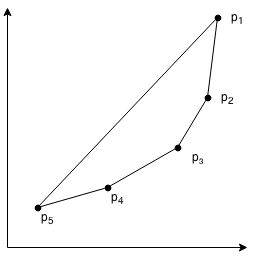
\includegraphics[width=5cm]{sketch1}
\end{center}
\caption{Konvexe Hülle}
\end{figure}

Beweis:\\
TODO

Somit könnte man den Polygonzug in linearer Zeit ablaufen um die sortierte Folge $a_n,..,a_1$ zu erhalten (da stets $x_i\ge x_{i+1}$). Das Sortieren der Folge hätte somit nur soviel Zeit benötigt wie die Konstruktion der konvexen Hülle zzgl. $O(n)$ für das Berechnen der Quadrate und noch einmal $O(n)$ für das Ablaufen des Polygonzugs. Dies ist nach Annahme jedoch nicht möglich: die Konstruktion der konvexen Hülle muss folglich $\Omega (n\cdot\log n)$ Zeit benötigen.
\end{task}
\end{document}